


\tikzset{every picture/.style={line width=0.75pt}} %set default line width to 0.75pt        

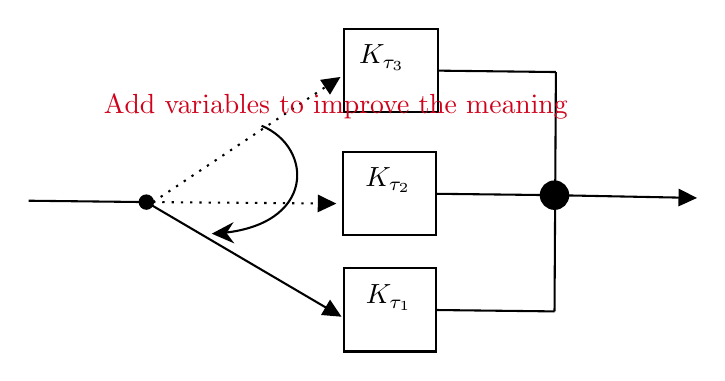
\begin{tikzpicture}[x=0.75pt,y=0.75pt,yscale=-1,xscale=1]
%uncomment if require: \path (0,300); %set diagram left start at 0, and has height of 300

%Straight Lines [id:da7325827417734325] 
\draw    (110.3,130.37) -- (166.97,131.03) ;
%Shape: Circle [id:dp2471826639953869] 
\draw  [fill={rgb, 255:red, 0; green, 0; blue, 0 }  ,fill opacity=1 ] (163.76,131.03) .. controls (163.76,129.26) and (165.2,127.83) .. (166.97,127.83) .. controls (168.74,127.83) and (170.17,129.26) .. (170.17,131.03) .. controls (170.17,132.8) and (168.74,134.24) .. (166.97,134.24) .. controls (165.2,134.24) and (163.76,132.8) .. (163.76,131.03) -- cycle ;
%Straight Lines [id:da9293679132290389] 
\draw    (166.97,131.03) -- (258.41,184.73) ;
\draw [shift={(261,186.25)}, rotate = 210.42] [fill={rgb, 255:red, 0; green, 0; blue, 0 }  ][line width=0.08]  [draw opacity=0] (8.93,-4.29) -- (0,0) -- (8.93,4.29) -- cycle    ;
%Straight Lines [id:da24281601207282866] 
\draw  [dash pattern={on 0.84pt off 2.51pt}]  (170.17,131.03) -- (255.5,131.73) ;
\draw [shift={(258.5,131.75)}, rotate = 180.46] [fill={rgb, 255:red, 0; green, 0; blue, 0 }  ][line width=0.08]  [draw opacity=0] (8.93,-4.29) -- (0,0) -- (8.93,4.29) -- cycle    ;
%Straight Lines [id:da8961600824558422] 
\draw  [dash pattern={on 0.84pt off 2.51pt}]  (170.17,131.03) -- (258,72.42) ;
\draw [shift={(260.5,70.75)}, rotate = 146.28] [fill={rgb, 255:red, 0; green, 0; blue, 0 }  ][line width=0.08]  [draw opacity=0] (8.93,-4.29) -- (0,0) -- (8.93,4.29) -- cycle    ;
%Straight Lines [id:da9497280508447912] 
\draw    (306.97,127.03) -- (363.63,127.7) ;
%Straight Lines [id:da7406136585517815] 
\draw    (306.97,183.03) -- (363.63,183.7) ;
%Straight Lines [id:da9889302923957719] 
\draw    (307.63,67.7) -- (364.3,68.37) ;
%Straight Lines [id:da43400533320140733] 
\draw    (364.3,68.37) -- (363.63,183.7) ;
%Shape: Circle [id:dp16791554484697713] 
\draw  [fill={rgb, 255:red, 0; green, 0; blue, 0 }  ,fill opacity=1 ] (357.03,127.7) .. controls (357.03,124.05) and (359.99,121.1) .. (363.63,121.1) .. controls (367.28,121.1) and (370.23,124.05) .. (370.23,127.7) .. controls (370.23,131.35) and (367.28,134.3) .. (363.63,134.3) .. controls (359.99,134.3) and (357.03,131.35) .. (357.03,127.7) -- cycle ;
%Straight Lines [id:da219741695471819] 
\draw    (363.63,127.7) -- (429.3,128.98) ;
\draw [shift={(432.3,129.03)}, rotate = 181.11] [fill={rgb, 255:red, 0; green, 0; blue, 0 }  ][line width=0.08]  [draw opacity=0] (8.93,-4.29) -- (0,0) -- (8.93,4.29) -- cycle    ;
%Shape: Rectangle [id:dp4766267400327753] 
\draw   (262,47.5) -- (307.5,47.5) -- (307.5,87.5) -- (262,87.5) -- cycle ;
%Shape: Rectangle [id:dp20249482055734336] 
\draw   (261.5,107) -- (306.5,107) -- (306.5,147) -- (261.5,147) -- cycle ;
%Shape: Rectangle [id:dp6220688812324011] 
\draw   (262,163) -- (306.5,163) -- (306.5,203) -- (262,203) -- cycle ;
%Curve Lines [id:da15451956461581107] 
\draw    (222.5,94.25) .. controls (247.49,104.54) and (248.95,142.68) .. (201.47,146.09) ;
\draw [shift={(198.5,146.25)}, rotate = 357.73] [fill={rgb, 255:red, 0; green, 0; blue, 0 }  ][line width=0.08]  [draw opacity=0] (10.72,-5.15) -- (0,0) -- (10.72,5.15) -- (7.12,0) -- cycle    ;

% Text Node
\draw (267.95,53.83) node [anchor=north west][inner sep=0.75pt]    {$K_{\tau _{3}}$};
% Text Node
\draw (271.28,169.5) node [anchor=north west][inner sep=0.75pt]    {$K_{\tau _{1}}$};
% Text Node
\draw (270.95,112.67) node [anchor=north west][inner sep=0.75pt]    {$K_{\tau _{2}}$};
% Text Node
\draw (145,77.5) node [anchor=north west][inner sep=0.75pt]  [color={rgb, 255:red, 208; green, 2; blue, 27 }  ,opacity=1 ] [align=left] {Add variables to improve the meaning};


\end{tikzpicture}